
\chapter{Ekonomické aspekty pandemie}\label{Ekonomicke_aspekty}

\textit{Eva Hromádková}
\vspace{15mm}

\section*{Úvod} 
Probíhající pandemie covid-19 a následná vládní opatření se od jara loňského roku promítají do společenského i ekonomického života. Dle předběžných odhadů Českého statistického úřadu se ekonomika v roce 2020 propadla o 5,6~\%\footnote{\url{https://www.czso.cz/csu/czso/cri/predbezny-odhad-hdp-4-ctvrtleti-2020}}, což byl největší pokles v historii samostatné České republiky. Je přitom důležité zmínit, že její výchozí situace byla v porovnání s jinými zeměmi postiženými pandemií relativně dobrá, s ohledem na relativně malou výchozí zadluženost veřejného sektoru, velmi nízkou úroveň nezaměstnanosti či limitovanou zadluženost soukromého sektoru. 

Ekonomický šok byl však velice silný a dá se předpokládat, že jeho dopady budou ještě dlouho doznívat. Na vážnost situace měla přitom nemalý vliv reakce vlády a veřejných institucí, které svou politikou a opatřeními mohly ekonomickou krizi zmírnit, jak se to i částečně podařilo na přelomu jara a léta, anebo naopak zhoršit -- viz neuvážené rozvolňování před Vánocemi nebo třeba nedbalý přístup k testování od počátku podzimu 2020.

Tento článek se ve své hlavní části zaměřuje na popis ekonomické situace v průběhu pandemie a na hrubý odhad ekonomických a sociálních nákladů, které s sebou přinesla. Strukturou sleduje práci \cite{Levy2021}, když v úvodu analyzuje vývoj ekonomiky a reakci jednotlivých jejích segmentů – domácností a podnikatelské sféry – na covid-19. V další části se zaměřuje na celkový dopad do veřejných financí a v posledních dvou zkoumá společenské a osobní náklady pandemie ve smyslu hodnoty ztracených životů (nadměrná úmrtí) i mezery ve vzdělávání v důsledku uzávěry škol. Následná diskuse se pokouší zhodnotit, do jaké míry se vhodnou ekonomickou politikou dalo jednotlivým typům nákladů vyhnout, případně je snížit.

\section*{Analýza ekonomických a sociálních dopadů pandemie covid-19} 

\subsection*{Růst ekonomiky} 
Propad ekonomické aktivity v České republice byl nepřekvapivě největší ve druhém čtvrtletí 2020 (-10,8 \%), v návaznosti na téměř úplný lockdown, tj. restrikce na pohyb obyvatel a dočasné omezení průmyslné výroby a jiných odvětví kromě kritických (Obrázek \ref{fig:110-HDP}). Po letním uvolnění, nedostatečné přípravě a nástupu dalších vln pandemie zůstala meziroční dynamika HDP až do prvního čtvrtletí 2021 pořád v záporu. Nejvíce k tomu přispělo opakované uzavření maloobchodu a služeb, tj. segmentů, které jsou těsně svázané se spotřebou domácností. 

\begin{figure}[ht]
    \centering
    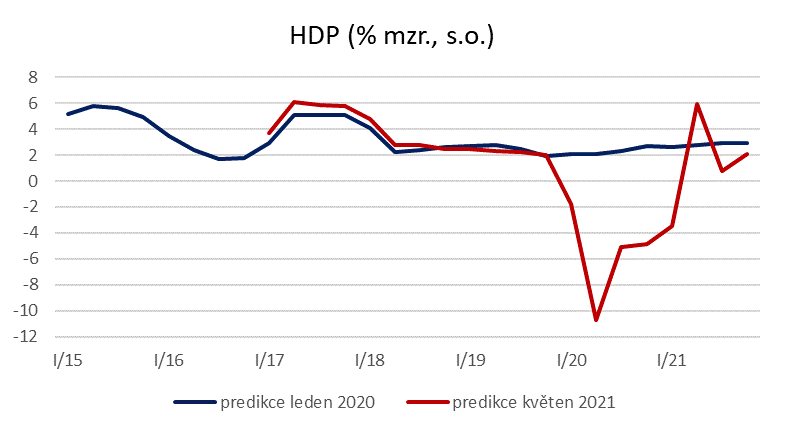
\includegraphics[width=0.49\textwidth]{./pic/HDP.png} \includegraphics[width=0.49\textwidth]{./pic/inflace.png}
    \caption{Srovnání prognózy hlavních ekonomických ukazatelů v situační zprávě České národní banky z ledna 2020 a května 2021. Zdroj: Prognóza ČNB (ČNB, 2020 a 2021)}
    \label{fig:110-HDP}
\end{figure} 

Samotné domácnosti se přitom dle barometru spotřebitelské nálady\footnote{\url{https://ec.europa.eu/info/business-economy-euro/indicators-statistics/economic-databases/business-and-consumer-surveys/download-business-and-consumer-survey-data/press-releases_en\#2020}} nejvíce obávaly vývoje na trhu práce a nezaměstnanosti. V této oblasti však relativně efektivně zafungovaly vládní podpůrné programy Antivirus a kompenzační bonus. Míra nezaměstnanosti se i díky tomu udržela na relativně nízké úrovni. Poklesla však míra za\-měst\-na\-nos\-ti, což naznačuje, že část populace řešila svůj problém celkovým odchodem z trhu práce (Obrázek \ref{fig:110-trhprace}). Domácnosti omezily svoji spotřebu a za poslední rok vygenerovaly dodatečné úspory ve výši 260 mld. Kč, což odpovídá 22 \% z disponibilního důchodu (pro srovnání, ve 4. čtvrtletí 2019 činila míra úspor 13 \%). 

\begin{figure}[ht]
    \centering
    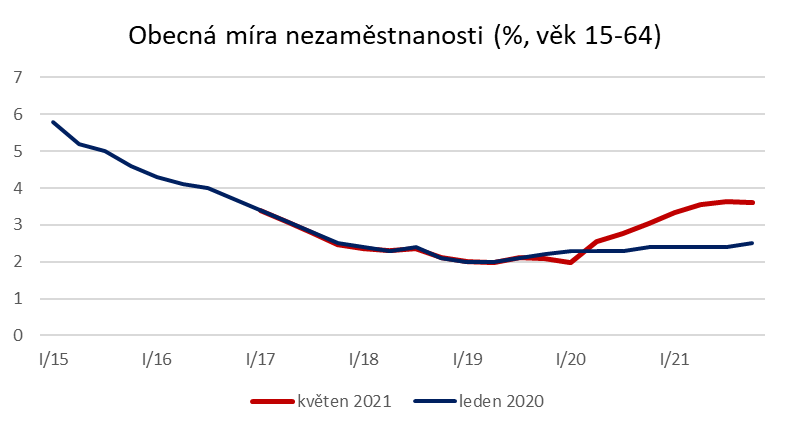
\includegraphics[width=0.49\textwidth]{./pic/nezamestnanost.png} 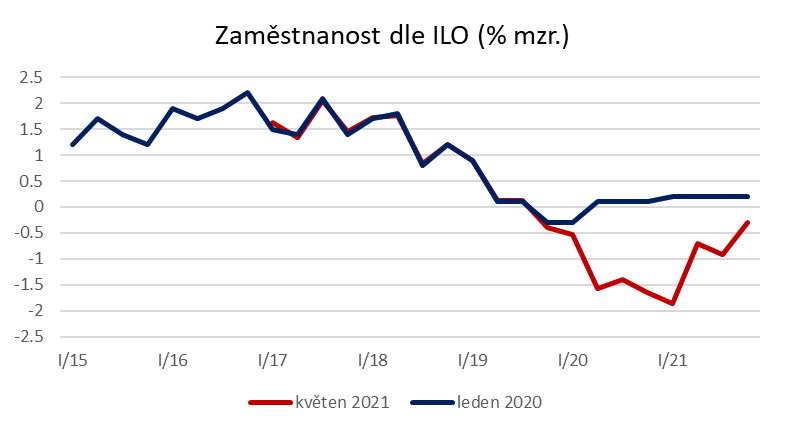
\includegraphics[width=0.49\textwidth]{./pic/zamestnanost.png}
    \caption{Srovnání prognózy hlavních ukazatelů trhu práce v situační zprávě České národní banky z ledna 2020 a května 2021. Zdroj: Prognóza ČNB (ČNB, 2020 a 2021)}
    \label{fig:110-trhprace}
\end{figure}

Rok 2020 byl tvrdý pro většinu firem a živnostníků v zemi. Dle vyjádření předsedy Hospodářské komory přerušilo svou živnost více než 130 tisíc živnostníků\footnote{\url{https://www.komora.cz/press_release/projev-vladimira-dlouheho-rok-od-prvniho-nouzoveho-stavu/}}. Paradoxně je počet bankrotů v porovnání s předešlými roky nižší, ale to souvisí se zavedením moratoria na podávání insolvenčních rozhodnutí a návrhů. Negativní dopady se však soustředily primárně na sektory maloobchodu a služeb. Průmyslu a navazujícím odvětvím se v posledním zhruba půlroce vyhýbaly. Až začátkem roku 2021 oslabil i průmysl včetně exportních odvětví, což bylo dáno narušením dodávek některých surovin, materiálů a komponent. Vysoká otevřenost české ekonomiky vůči zahraničí, která v kritickém období skrze vývoz produkci podporovala, se tak stává brzdícím činitelem – vývoz stagnuje z důvodu chybějících vstupů a dovoz jako důsledek malé domácí poptávky.

Celkově byl propad HDP za rok 2020 odhadnut na -5,6 \% tj. téměř 7 procent níže, než bylo predikováno před nástupem pandemie. I když prognóza ČNB, MFČR i jiných institucí očekává pro tento rok výrazný překmit do pozitivních čísel, je tomu tak jenom z důvodu nízké srovnávací základny a růst je podmíněn uvolněním opatření s účinností od třetího čtvrtletí až do konce roku. Zároveň se společnost bude společnost potýkat s projevy vyšší inflace (už teď se dle anekdotické evidence zdvihli ceny piva v restauracích o 10 \%), a po zrušení podpůrných programů i se zhoršující se situací na trhu práce. Jestli tyto efekty rychle pominou, záleží na rychlosti zotavování našich obchodních partnerů (zejména Německa), jako i na promyšlenosti strategie hospodářské politiky vlády. Ve volebním roku se ale dají očekávat spíše populistické kroky směrem k nejovlivnitelnější části voličské populace, viz plánovanou valorizaci důchodů.

\subsection*{Fiskální stimul} 
Hluboký propad ekonomické aktivity ovlivnil hospodaření veřejných rozpočtů skrze dva hlavní kanály. Prvním je pokles daňových a pojistných příjmů, druhým pak stimulační opatření přijímaná vládou, která mohou být zaměřena jak na příjmovou (snižování daní), tak na výdajovou stranu veřejných rozpočtů (nové výdajové programy). 

O ex ante kvantifikaci poklesu daňových a pojistných příjmů se mimo jiné pokusila Národní rozpočtová rada (\cite{Hlavacek2020}), která ve svém výpočtu vycházela z odhadu tzv. produkční mezery, tj. o kolik méně se v ekonomice vyprodukuje v porovnání s optimálním stavem (tzv. potenciálem). Propad růstu HDP za rok 2020 o 5,8 \% by přitom implikoval výpadek příjmu v přibližné hodnotě 165 mld. Kč. Tato prognóza z dubna 2020 se skoro přesně naplnila, když pokles daňových příjmů za rok 2020 činil cca 2,7 \% (\cite{MFCR2021}), přičemž nejvíce se propadl výnos daně z příjmů právnických osob (-22,1 \%).

Vedle propadu příjmů ale k nárůstu deficitu veřejných rozpočtů přispěla i diskreční opatření vlády k podpoře domácí ekonomiky a zaměstnanosti. \cite{Hlavacek2020} ve své zprávě kvantifikovali dopady těch kroků vlády, které měly zásadnější dopad do veřejných rozpočtů pro rok 2020 a 2021. Do těchto opatření přitom nezahrnovali opatření týkající se regulace ekonomicko-právních vazeb (např. odklad placení nájmu, odklad splátek bankovních i nebankovních úvěrů) ani budoucí náklady spojené s poskytnutými zárukami na úvěry či odkladem placení daní. Celkové výdaje na tato diskreční opatření byly koncem roku 2020 odhadovány na přibližně 160 mld. Kč, přičemž největší podíl na vynaložených prostředcích má program podpory zaměstnanosti Antivirus (17 \%), kompenzační bonus (15 \%) a jednorázový příspěvek důchodcům (9 \%). Diskreční výdaje přitom pokračují i v roce 2021, přičemž některé programy byly prodlouženy (COVID 2021), některé jsou zavedeny nově (testování dětí ve školách) a u některých se zvyšovaly příspěvky (ošetřovné).

Důležitou součástí diskuse o nastavení diskrečních opatření bylo vedle jejich objemu také načasování a zaměření. Už od začátku pandemie se ze strany předních českých ekonomů ozývaly hlasy volající po včasných (lépe řečeno okamžitých) a cílených opatřeních na podporu nejohroženějších skupin spo\-le\-čno\-sti. Odpověď vlády byla většinou zpožděná (např. u bonusu pro lidi v karanténě, schváleného 4. března 2021, tj. rok po začátku pandemie), neúplná a nepřesně zaměřená, v některých případech pak těžce dosažitelná pro cílovou skupinu (např. COVID – kultura). Zároveň se platnost opatření po nezvládnutém nástupu druhé, třetí a čtvrté vlny pandemie musela prodlužovat, čímž se náklady dále zvyšovaly.

\begin{figure}[ht]
    \centering
    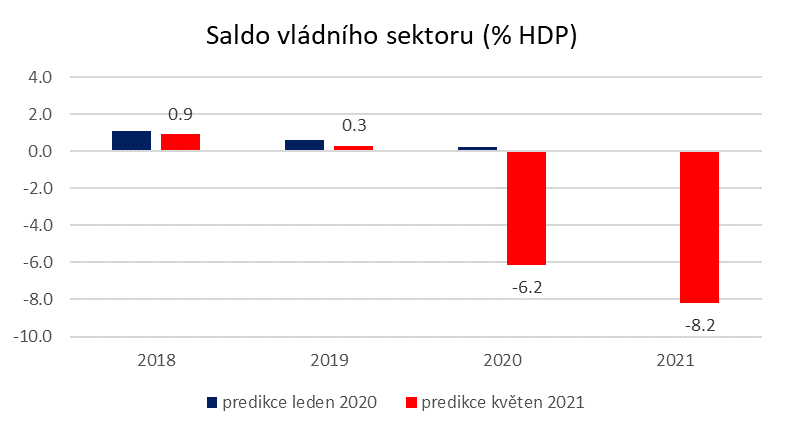
\includegraphics[width=0.49\textwidth]{./pic/saldo.png} 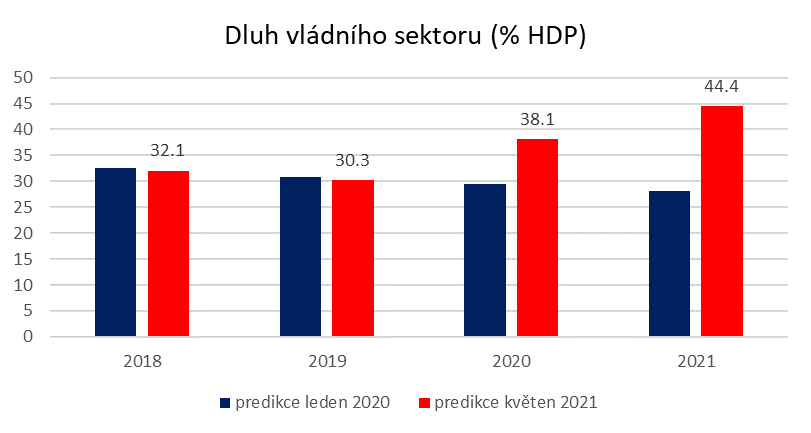
\includegraphics[width=0.49\textwidth]{./pic/dluh.png}
    \caption{Srovnání prognózy salda a dluhu vládního sektoru, v situační zprávě České národní banky z ledna 2020 a května 2021. Zdroj: Prognóza ČNB (ČNB, 2020 a 2021)}
    \label{fig:110-vlada}
\end{figure}

Kombinace výpadku příjmů a vysokých výdajů v roce 2020 vedla ke skokovému nárůstu vládního deficitu (saldo -6,2 \% HDP), jakož i vládního dluhu (růst z 30,3 \% v 2019 na 38,1 \% v roce 2020). Před nástupem pandemie se přitom po mírném přebytku v předešlých letech očekávala pro roky 2020 a 2021 vyrovnaná bilance, s ohledem na očekávané výdaje spojené s volebním rokem (pro srovnání prognózy z doby před začátkem pandemie a aktuální prognózy viz Obrázek fig:110-vlada). Pokračující epidemie se odrazí i v letošním saldu, které se očekává meziročně ještě hlubší (prognóza ČNB je -8,2 \% HDP, zatímco MF ČR očekává – 8,8 \%). Zadlužení veřejných financí pak v tomto scénáři vzroste z 38,1 \% HDP v roce 2020 na 44,4 \% HDP ke konci roku 2021. Tak vysoké hodnoty zadlužení budou vést k nutnosti konsolidace veřejných financí, a to buď cestou omezení výdajů (což ale v současnosti vzhledem k populistickým plánům valorizace důchodů a navýšení příspěvků na děti není reálné), nebo zvýšení příjmů ze zdanění (\cite{NRR2021}). Restriktivní fiskální politika se zákonitě odrazí v nižším ekonomickém růstu do budoucna.

\subsection*{Hodnota nadměrných úmrtí:} 

Snížená ekonomická aktivita není jediným ekonomickým nákladem pandemie covid-19. Asi nejkontroverznějším tématem v tomto ohledu je peněžní ohodnocení s covidem souvisejících úmrtí, jakož i snížené kvality života některých pacientů po prodělání covidu. Kontroverze spočívá ve dvou oblastech: zaprvé vzhledem k různým postupům vykazování příčin úmrtí i napříč jednotlivými nemocnicemi v České republice je statistika oficiálních úmrtí na covid-19 nepřesná. Neprojeví se v ní ani špatně diagnostikovaní (a netestovaní) pacienti ani nepřímá úmrtí v důsledku zanedbání péče při přehlceném zdravotnickém systému. Proto se jako nejpřesnější přístup ukazuje definice tzv. nadměrných úmrtí, tedy rozdíl počtu lidí, kteří ve stejném období zemřeli v České republice v předcházejících letech, s počtem zemřelých v době pandemie. 

\cite{Karlinsky2021} ve své studii mapující nadměrnou úmrtnost v 81 státech světa odhadují, že v ČR zemřelo v roce 2020 o 20 tisíc lidí více (tj. 18 \%) než za průměr posledních pěti let. Pro srovnání, počet úmrtí v souvislosti s nemocí covid-19 podle oficiálních statistik\footnote{\url{https://onemocneni-aktualne.mzcr.cz/covid-19}} za rok 2020 činí kolem 12 tisíc. V současnosti (začátek června 2021) se oficiální počet úmrtí přehoupl přes 30 tisíc, což Českou republiku v mezinárodním srovnání řadí na čtvrtou příčku za Peru, Maďarsko, a Bosnu a Hercegovinu\footnote{\url{https://ourworldindata.org/}}. V metrice nadměrných úmrtí tak celkem můžeme očekávat více než 50 000 ztracených životů.

Druhou problematickou oblastí je ekonomické ohodnocení nadměrných úmrtí, jelikož myšlenka, že lidský život se dá ocenit penězi, je pro mnohé nepřijatelná. V oblasti ekonomie zdravotnictví se proto pracuje s konceptem tzv. hodnoty statistického života, která měří, jak moc jsou lidé ochotní zaplatit za možnost redukovat či odstranit riziko úmrtí. Liší se tak od přístupu, kdy je život člověka hodnocen na základě jeho budoucích příjmů, a proto taky neklesá s věkem, nižším příjmem apod \footnote{\url{https://www.theregreview.org/2020/08/05/robinson-covid-19-uncertainties-value-statistical-life/}}. Odhady využívané americkými regulátory pro posouzení efektivity nových léčebných postupů operují s hodnotami mezi 7 a 10 miliony USD, tj. minimálně 150 mil. Kč, což by při současném počtu úmrtí znamenalo celkem 7,5 bilionu Kč. Třeba si však uvědomit, že hodnota statistického života se v praxi používá zejména na cost-benefit analýzu, tj. srovnání, jak velké výdaje jsou stále akceptovatelné pro záchranu životů.

Dalším nezanedbatelným nákladem je snížení kvality života těch pacientů, kteří covid-19 překonali, a vyvinula se u nich dlouhodobá komplikace. Data z epidemie SARS ukazují, že přibližně jedna třetina pacientů, kteří měli vážnou formu onemocnění, trpí souvisejícími chronickými potížemi. Na základě tohoto předpokladu a odhadu následného snížení kvality života o cca 35 \% pak \cite{Cutler2020} vyčíslili hodnotu těchto potíží na přibližně jednu polovinu hodnoty ztracených životů. V České republice by to zodpovídalo 3,8 bilionu Kč, co pořád nezahrnuje náklady související s dopady na mentální zdraví populace, viditelné ve zvýšení prevalence depresí a úzkostí.

\subsection*{Efekt školských uzávěr:} 

Poslední oblastí, kterou se při kvantifikaci ekonomických důsledků pandemie budu zaobírat, je školství. Empirické studie dopadů dávnějších školních výluk, absencí, jakož i několik dopadových studií přímo zaměřených na výluky z období pandemie covid-19 (přehled v \cite{Jann2021}) implikují, že výluka prezenční výuky bude mít výrazné negativní dopady na úroveň vzdělanosti a školní výsledky žáků. To se promítne i do budoucích výdělků současných žáků a studentů v celém průběhu jejich pracovního života. Česká republika má přitom podle dat UNESCO ze zemín EU nejdelší reportovanou celkovou délku uzávěry škol (47 týdnů), když obdobně jsou na tom Slovensko (46 týdnů) a Polsko (43 týdnů), naproti tomu stojí Francie s 12, případně Španělsko s 15 týdny\footnote{\url{https://en.unesco.org/covid19/educationresponse\#durationschoolclosures}}.

\cite{Jann2021} vyčíslili soukromé náklady (pro žáky a studenty) jednoho týdne absolutní výluky školní výuky v České republice na 50 mld. Kč a dalších 16 mld. veřejných nákladů z titulu ušlých budoucích příjmů veřejných rozpočtů z pojistných odvodů zaměstnavatelů, tj. celkem 66 mld. Kč za týden. Za předpokladu, že distanční výuka nahradí v průměru 50 \% prezenční výuky, je tak odhadována ztráta 33 mld. Kč týdně, tj. cca 660 mld. za výluku v délce poloviny školního roku. To představuje přibližně 12 \% českého HDP za rok 2020, přičemž ke stejnému podílu, jenom na globálním HDP, se dostala i studie \cite{Azevedo2020}. Výše uvedené přímé ztráty v podobě ušlých budoucích výdělků v sobě ale nezahrnují sekundární náklady rodičů, kteří museli omezit svou pracovní činnost z důvodu péče o děti, ani absenci jiných externalit spojených s vyšším vzděláním.

\section*{Diskuse:} 
Z hrubé kvantifikace uvedené v článku je zřejmé, že ekonomické a sociální náklady pandemie covid-19 budou vysoké, a to jak v krátkodobém, tak v dlouhodobém horizontu. V ex post pohledu a s možností srovnání výsledků s jinými zeměmi se přitom dá vcelku objektivně posoudit, které z těchto nákladů byly neodvratné a kterým se dalo vhodnou hospodářskou politikou a strategickým managementem krize předejít.

Mezi nevyhnutelné náklady patří zejména náklady prvotního lockdownu, jelikož se odehrál v situaci, kdy téměř nikdo na světě neměl dostatek informací o nebezpečí, které virus představuje. Svoje ekonomiky uzavřely téměř všechny země světa, a omezil se nejen cestovní ruch, ale i mezinárodní obchod. Jelikož velká část české produkce směřuje do zahraničí a je zároveň dovozně náročná, epidemiologický vývoj a následná regulační opatření v jiných zemích je třeba také považovat za exogenní, a náklady z nich plynoucí za nevyhnutné. Další položkou, která se ex post jeví jako z větší míry oprávněná, jsou výdaje na opatření pro zmírnění důsledků koronaviru z veřejných financí. V případě tohoto typu krize je nutné, aby byla pomoc okamžitá a cílená, aby se jasně komunikoval očekávaný výsledek. Některé výdajové položky jsou však z tohoto pohledu sporné, jako např. jednorázový příspěvek seniorům začátkem záři, u nějž se o včasnosti rozhodně nedá mluvit.

Naopak náklady spojené s ekonomickými důsledky druhé, třetí a čtvrté vlny pandemie v České republice se dají považovat za důsledky nevhodné strategie přípravy a přijímání opatření v oblasti zdravotnictví, školství, financí i hospodářství. Smutný fakt, že Česká republika je jednou z nejzasaženějších zemí, co se týče počtu úmrtí, že tady byla nejdéle omezována prezenční školní docházka, nebo že český zdravotnický systém v únoru téměř narazil na limity svého fungování, naznačují, že přijatá rozhodnutí byla neefektivní nebo zpožděná (například testování v práci a školách). Přitom již velice jednoduché modely šíření epidemie, jejichž výsledky byly v rámci činnosti IDEA COVID-19 prezentovány na konferenci v půlce května 2020, ukazovaly, že existuje alternativa k plošným uzávěrám – důsledné trasování všech identifikovaných kontaktů a karanténa. V současnosti se nejefektivnější cestou pro potlačení viru stálo očkování. 
